\documentclass[11pt,twocolumn]{scrartcl}

\usepackage{natbib}
\bibliographystyle{plain}

\usepackage{tikz}
\usetikzlibrary{bayesnet}

\author{
    Verdegaal Jacob \\
    \texttt{jacob.verdegaal@student.uva.nl}
    \and
    Drumm, Eli\\
    \texttt{etd@dte.li}
    \and
    Noble, Bill\\
    \texttt{winobes@gmail.com}
}

\title{Inducing Semantic Frames on a Very Large Corpus of Syntactic-Ngrams}

\renewcommand\phi\varphi

\begin{document}

\maketitle

\begin{abstract}
This is the abstract which we will write.
\end{abstract}



\section{Introduction}
Here we provide some background information about what are semantic frames and 
what it menas to induce them and stuff like that.


\section{Related Work}
Here we talk mostly about the O'Connor paper \cite{oconnor2013} and the Rooth 
paper \cite{rooth1999}.


\section{Induction Models}

\subsection{Model 0: Un-structured Tuples}
\begin{figure}
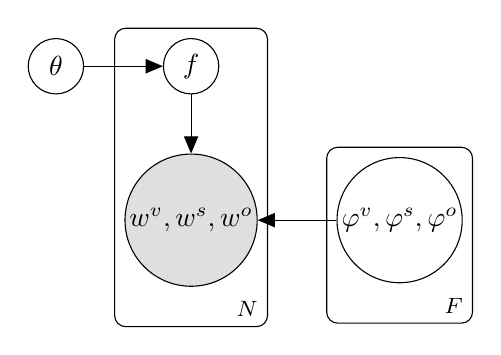
\begin{tikzpicture}
  % Nodes
  \node[obs] (datapoint) {$w^v,w^s,w^o$} ; %
  \node[latent, above=0.75cm of datapoint] (F) {$f$} ; %
  \node[latent, left=of F] (theta) {$\theta$}; %
  \node[latent, right=of datapoint] (phi) {$\varphi^v,\varphi^s,\varphi^o$}; %
  \edge {theta} {F} ; %
  \edge {F} {datapoint}
  \edge {phi} {datapoint} ; %
  \plate {tuples} {(F) (datapoint) } {$N$}; %
  \plate {} {(phi)} {$F$} ; %
\end{tikzpicture}

\caption{Model 0}
\end{figure}

\subsection{Model 1: Verb Documents}
\begin{figure}
    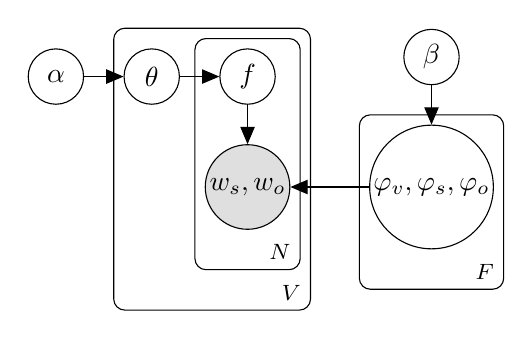
\begin{tikzpicture}[]
    \node[obs]                   (w)     {$w_s,w_o$}; %
    \node[latent, above=0.5cm of w]     (f)     {$f$};
    \node[latent, left=0.5cm of f]     (theta) {$\theta$};
    \node[latent, left=0.5cm of theta] (alpha) {$\alpha$};
    \node[latent, right=of w]    (phi)   {$\varphi_v,\varphi_s,\varphi_o$};
    \node[latent, above=0.5cm of phi] (beta) {$\beta$};
    \edge {alpha} {theta};
    \edge {theta} {f};
    \edge {f} {w};
    \edge {phi} {w};
    \edge {beta} {phi};
    \plate {frames} {(phi)} {$F$};
    \plate {datapoints} {(f) (w)} {$N$};
    \plate {verbs} {(f) (w) (datapoints) (theta)} {$V$};
\end{tikzpicture}

    \caption{Model 1}
\end{figure}


\section{Data}

\subsection{Google Syntactic-ngrams}
Here we talk a bit about the syntactic n-grams and all that \cite{ngrams2013}.

\subsection{Pruning}


\section{Experiments}


\section{Results}


\section{Discussion}


\section{Future Work}


\section{Conclusion}


\bibliography{refs.bib}
\end{document}
